\section{Question 1}

$X$ is a continuous-valued random variable with uniform density in $(-1, +1)$. 

\subsection{Item a}
Draw its probability density function (PDF). What is the area under the curve? Justify your answer.

\subsection{Item b}
Draw its cumulative distribution function (CDF).

\subsection{Item c}
Calculate the probability of the event $X\in(-0.2, 0.2)$.

\subsection{Item d}
Calculate the expected value $\E[X]$, 
the second $\E[X^2]$ and the fourth moment $\E[X^4]$ of the random variable. 
Calculate its variance $\var[X]$, as well.

\noindent\rule{\textwidth}{.5pt}

Let $p: \mathbb{R} \to \mathbb{R}$ denote the PDF of $X$ 
and $c: \mathbb{R} \to \mathbb{R}$ its CDF.
Since the random variable is of uniform density in $(-1, +1)$, 
%
\begin{equation}
    p(x) = \begin{cases}
        k, & |x| < 1 \\
        0, & |x| \geq 1
    \end{cases}
\end{equation}
%
for some constant $k > 0$.
%
By definition, the area under the PDF curve is equal to the probability $P$ of $X$ assuming a value in the associated range $(a, b)$,
$P(a < X < b) = \int_a^b p(x) \ dx$.
%
For $a=-\infty$ and $b=\infty$,
$P(-\infty < X < \infty) = 1$, i.e., the probability of $X$ assuming \textit{any} value is 100\%.
We can use this result (in general, an identity) to find the value of $k$:
%
\begin{align}
    P(-\infty < X < \infty) = \int_{-\infty}^\infty p(x) \ dx = 1 
    \implies
    \int_{|x| \geq 1} p(x) \ dx + 
    \int_{|x| < 1} p(x) \ dx & = 1
    \\
    \int_{|x| \geq 1} 0 \ dx + 
    \int_{|x| < 1} k \ dx & = 1
    \\
    2k &= 1 \quad\therefore\quad 
    k = \frac{1}{2}.
\end{align}

With $k$ evaluated, we can find any $P$, e.g., 
$P(-0.2 < X < 0.2) = [0.2-(-0.2)] \cdot (1/2) = 0.2$.
A drawing of $p(x)$ and $c(x) = \int_{-\infty}^x p(z)\ dz$ is presented in \cref{fig:pdf-cdf}.
%
\begin{figure}[htbp]
    \centering
    \caption{PDF and CDF of a uniform distribution in $(-1, 1)$.}
    \label{fig:pdf-cdf}
    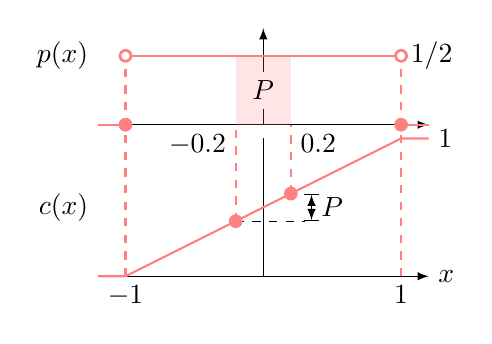
\begin{tikzpicture}[> = latex, scale=1.75]
    \def\r{0.05}
    % PDF
    %% Axis
    \draw [->] (-1.2, 0) -- (1.2, 0);
    \draw [->] (0, 0) -- (0, 0.7);
    %% Curve
    \fill [red!50, opacity=0.2]
        (-0.2, 0) rectangle (0.2, 0.5);
    \node [fill=red!10] at (0, 0.25) {$P$}; 
    \draw [thick, red!50] 
    (-1.2, 0) -- (-1, 0)
    (-1, 0.5) -- (1, 0.5) 
    (1, 0) -- (1.2, 0);
    %% Decorations
    \fill [red!50] 
        (-1, 0.5) circle (\r)
        (1, 0.5) circle (\r)
        (-1, 0) circle (\r)
        (1, 0) circle (\r);
    \fill [white] 
        (-1, 0.5) circle (\r-0.02)
        (1, 0.5) circle (\r-0.02);
    %% Annotations
    \draw 
        (1, 0.5) node [right] {$1/2$}
        (-0.2, 0) node [below left] {$-0.2$}
        (0.2, 0) node [below right] {$0.2$}
        (-1.2, 0.5) node [left] {$p(x)$};
        
    % CDF 
    \begin{scope}[shift={(0, -1.1)}]
    %% Axis
    \draw [->] (-1.2, 0) -- (1.2, 0) node [right] {$x$};
    \draw (0, 0) -- (0, 1);
    %% Curve
    \draw [thick, red!50] (-1.2, 0) -- (-1, 0) -- (1, 1) -- (1.2, 1);
    %% Decorations
    \draw [thick, red!50, dashed]
        (-1, 0) -- (-1, 0.5 +1.05)
        (1, 0) -- (1, 0.5 +1.05)
        (-0.2, 0.4) -- (-0.2, 1.1)
        (0.2, 0.6) -- (0.2, 1.1);
    %% Annotations
    \draw
        (-1, 0) node [below] {$-1$}
        (1, 0) node [below] {$1$}
        (1.2, 1) node [right] {$1$}
        (-1.2, 0.5) node [left] {$c(x)$};
    \draw [dashed] (-0.2, 0.4) --++ (0.5, 0);
    \fill [red!50] 
        (-0.2, 0.4) circle (\r)
        (0.2, 0.6) circle (\r);
    \draw [ |<->| ] (0.2 +0.15, 0.6) --++ (0, -0.2) node [midway, right] {$P$};
    \end{scope}
\end{tikzpicture}
\end{figure}

Next, the variance and some of the moments of $p$ is calculated.
By definition, 
$\E[X^n] = \int_\mathbb{R} x^n p(x)\ dx$. 
For this question's distribution,
%
\begin{align}
    \E[X^n] = \int_{-1}^1 x^n \cdot \frac{1}{2}\ dx
    = \frac{1}{2} \cdot \frac{x^{n+1}}{n+1}\bigg|_{x=-1}^{x=1}
    = \frac{1 + (-1)^n}{2(n+1)}
    = \begin{cases} 
        0, & n \text{ odd}\\
        1/(n+1), & n \text{ even}
    \end{cases}
\end{align} 

The above expression gives, for example, 
$\E[X]=0$, $\E[X^2]=1/3$, and $\E[X^4]=1/5$.
% 
As for the variance, the definition
$\var[X] = \E[(X - \E[X])^2] 
         = \E[X^2] - \E[X]^2$ 
results in $\var[X] = 1/3$.